%%%%%%%%%%%%%%%%%%%%%%%%%%%%%%%%%%%%%%%%%%%%%%%%%%%%%%%%%%%%%%%%%%%%%
%
%  This is a sample LaTeX input file for your contribution to
%  the MC2013 conference. Modified by R.C. Martineau at INL from A.
%  Sood at LANL, from J. Wagner ORNL who obtained the original class
%  file by Jim Warsa, LANL, 16 July 2002}
%
%  Please use it as a template for your full paper
%    Accompanying/related file(s) include:
%       1. Document class/format file: mc2013.cls
%       2. Sample Postscript Figure:   figure.eps
%       3. A PDF file showing the desired appearance: template.pdf
%    Direct questions about these files to: richard.martinea@inl.gov
%
%    Notes:
%      (1) You can use the "dvips" utility to convert .dvi
%          files to PostScript.  Then, use either Acrobat
%          Distiller or "ps2pdf" to convert to PDF format.
%      (2) Different versions of LaTeX have been observed to
%          shift the page down, causing improper margins.
%          If this occurs, adjust the "topmargin" value in the
%          mc2013.cls file to achieve the proper margins.
%
%%%%%%%%%%%%%%%%%%%%%%%%%%%%%%%%%%%%%%%%%%%%%%%%%%%%%%%%%%%%%%%%%%%%%


%%%%%%%%%%%%%%%%%%%%%%%%%%%%%%%%%%%%%%%%%%%%%%%%%%%%%%%%%%%%%%%%%%%%%
\documentclass{mc2013}
%
%  various packages that you may wish to activate for usage
\usepackage{graphicx}
\usepackage{tabls}
\usepackage{afterpage}
\usepackage{cites}
\usepackage{amsmath}
\usepackage{amssymb}
\usepackage{listings}
\usepackage{float}
\usepackage{caption}
\usepackage{subcaption}
\usepackage{verbatim}

\usepackage{tgheros}
\usepackage{xcolor}
\lstset {
    basicstyle=\sffamily
    breaklines=true
    language=C++,
    backgroundcolor=\color{black!5}, % set backgroundcolor
    basicstyle=\footnotesize,% basic font setting
    columns = flexible
}

%\usepackage{epsf}
%
%
% Insert authors' names and short version of title in lines below
%
\newcommand{\authorHead}      % Author's names here
   {A. Alfonsi, C. Rabiti, D. Mandelli, J.J. Cogliati, R.A. Kinoshita}
\newcommand{\shortTitle}      % Short title here
   {RAVEN as a tool for Dynamic Probabilistic Risk Assessment: Software Overview}
%%%%%%%%%%%%%%%%%%%%%%%%%%%%%%%%%%%%%%%%%%%%%%%%%%%%%%%%%%%%%%%%%%%%%
%
%   BEGIN DOCUMENT
%
%%%%%%%%%%%%%%%%%%%%%%%%%%%%%%%%%%%%%%%%%%%%%%%%%%%%%%%%%%%%%%%%%%%%%
\begin{document}

%
%      Headers and Footers
\afterpage{%
\fancyhf{}%
\fancyhead[CE]{
{\scriptsize \authorHead}}
\fancyhead[CO]{
{\scriptsize \shortTitle}}
%\lfoot{\scriptsize{
%International Conference on Mathematics and Computational Methods
%Applied to Nuclear Science \& Engineering (M\&C 2013),
%\\ Sun Valley, Idaho, USA, May 5-9, 2013.}}%
\rfoot{\thepage/\totalpages{}}%

\pagestyle{fancy}
%\setlength{\topmargin}{-20pt}
}

\normalsize

%\setlength{\baselineskip}{16.8pt}
\vspace{-3pt}

%
% TITLE
%

\begin{center}
\textbf{\large \\%
RAVEN AS A TOOL FOR DYNAMIC PROBABILISTIC RISK ASSESSMENT: SOFTWARE OVERVIEW
}
%
% FIRST AUTHORS
%


\setlength{\baselineskip}{14pt}
\textbf{A. Alfonsi, C. Rabiti, D. Mandelli, J.J. Cogliati, R.A. Kinoshita} \\ %\footnote{Footnote, if necessary, in Times New Roman font and font size 9}
Idaho National Laboratory  \\
2525 Fremont Avenue, Idaho Falls, ID 83415 \\
\{andrea.alfonsi, cristian.rabiti, diego.mandelli, joshua.cogliati, robert.kinoshita\}@inl.gov \\

\end{center}

%
% SET RAGGED RIGHT MARGIN
%
%\raggedright


\section*{ABSTRACT}
\begin{quote}
\begin{small}
RAVEN is a software tool under development at the Idaho National Laboratory (INL) that acts as the control logic driver and post-processing tool for the newly developed Thermal-Hydraulic code RELAP-7.
The scope of this paper is to show the software structure of RAVEN and its utilization in connection with RELAP-7. A short overview of the mathematical framework behind the code is presented along with its main capabilities such as on-line controlling/monitoring and Monte-Carlo sampling.
A demo of a Station Black Out PRA analysis of a simplified Pressurized Water Reactor (PWR) model is shown in order to demonstrate the Monte-Carlo and clustering capabilities.

\emph{Key Words}: Reactor Simulation, Probabilistic Risk Assessment, Dynamic PRA, Monte-Carlo, RELAP-7 %, Three Miles Island,
\end{small}
\end{quote}

\setlength{\baselineskip}{14pt}
\normalsize

%%%%%%%%%%%%%%%%%%%
\Section{INTRODUCTION}
%%%%%%%%%%%%%%%%%%%


RAVEN (\textbf{R}eactor \textbf{A}nalysis and \textbf{V}irtual control \textbf{EN}viroment)~\cite{ravenFY12,mandelliANS2012} is a software tool that acts as the control logic driver for the newly developed Thermal-Hydraulic code RELAP-7  (\textbf{R}eactor \textbf{E}xcursion and \textbf{L}eak \textbf{A}nalysis \textbf{P}rogram). The goal of this paper is to highlight the software structure of the code and its utilization in conjunction with RELAP-7. RAVEN is a multi-purpose \textbf{P}robabilistic \textbf{R}isk \textbf{A}ssessment (PRA) software framework that allows dispatching different functionalities.
It is designed to derive and actuate the control logic required to simulate the plant control system and operator actions (guided procedures) and to perform both Monte-Carlo sampling of random distributed events and event tree based analysis.
In order to facilitate the input/output handling, a \textbf{G}raphical \textbf{U}ser \textbf{I}nterface (GUI) and a post-processing data mining module, based on dimensionality and cardinality reduction, are available.
This paper wants to provide an overview of the software, highlighting the mathematical framework from which its structure is derived and showing a demo of a \textbf{S}tation \textbf{B}lack \textbf{O}ut (SBO) analysis of a simplified \textbf{P}ressurized \textbf{W}ater \textbf{R}eactor (PWR) model.

%%%%%%%%%%%%%%%%%%%%%%%%%%%%
\Section{MATHEMATICAL FRAMEWORK}
%%%%%%%%%%%%%%%%%%%%%%%%%%%%
\label{sec:mathFramework}

In this section the mathematical framework is briefly described by analyzing the set of the equations needed to model the control system in a nuclear power plant.

\Subsection{Plant and Control System Model}
\label{sec:PlantControlModel}
The first step is the derivation of the mathematical model representing, at a high level of abstraction, both
the plant and the control system models. In this respect, let be $\bar{\theta}(t)$ a vector describing the plant status in the phase space; the dynamic of both plant and control system can be summarized by the following equation:
\begin{equation}
\frac{\partial \bar{\theta}}{\partial t} = \bar{H}(\theta(t),t)
\label{eq:SystemDynamics}
\end{equation}
In the above equation we have assumed the time differentiability in the phase space. This is generally
not required and it is used here for compactness of notation. Now an arbitrary decomposition of the
phase space is performed:
\begin{equation}
\bar{\theta}=\binom{\bar{x}}{\bar{v}}
\label{eq:firstDecomposition}
\end{equation}
The decomposition is made in such a way that $\bar{x}$ represents the unknowns solved by RELAP-7, while $\bar{v}$ are the variables directly controlled by the control system (i.e., RAVEN). Equation~\ref{eq:SystemDynamics} can now be rewritten as follows:
\begin{equation}
\begin{cases}
\dfrac{\partial \bar{x}}{\partial t} = \bar{F}(\bar{x},\bar{v},t) \\
\dfrac{\partial \bar{v}}{\partial t} = \bar{V}(\bar{x},\bar{v},t) \\
\end{cases}
\label{eq:generalSystemEquation}
\end{equation}
As a next step, it is possible to note that the function
$\bar{V}(\bar{x},\bar{v},t)$
representing the control system, does not depend on the knowledge of the complete status of the system but on a restricted subset that we call control variables $\bar{C}$:
\begin{equation}
\begin{cases}
\dfrac{\partial \bar{x}}{\partial t} = \bar{F}(\bar{x},\bar{v},t) \\
\bar{C} = \bar{G}(\bar{x},t) \\
\dfrac{\partial \bar{v}}{\partial t} = \bar{V}(\bar{x},\bar{v},t)
\end{cases}
\label{eq:generalSystemEquationwithControl}
\end{equation}

%Note that even if it seems more appropriate, the standard naming of signals (monitored) and status (controlled) is not yet used. The reason for this choice is that, the chosen naming better mirrors the computational pattern between RAVEN and RELAP 7 and moreover the definition of signals is more tight to the definition of the control logic for each component and therefore relative rather than absolute in the overall system analysis. In fact we could have signal for a component that are status of another creating a definition that would be not unique. Another reason is that the standard naming will loose every meaning once used also for uncertainty analysis.

%%%%%%%%%%%%%%%%%%%%%%%%%%%%%%
\Subsection{Operator Splitting Approach}
%%%%%%%%%%%%%%%%%%%%%%%%%%%%%%
\label{sec:operatorSplitting}

The system of equations in Eq.~\ref{eq:generalSystemEquationwithControl} is fully coupled and in the past it has commonly been solved with an operator splitting approach. The reasons for this choice are several:
\begin{itemize}
\item Control system reacts with an intrinsic delay
\item The reaction of the control system might move the system between two different discrete states and
therefore numerical errors will be always of first order unless the discontinuity is treated explicitly.
\end{itemize}
RAVEN as well is using this approach (Fig.~\ref{fig:ControlSoftwareLayout}) to solve Eq.~\ref{eq:generalSystemEquationwithControl} which it becomes:
\begin{equation}
\begin{cases}
\dfrac{\partial \bar{x}}{\partial t} = \bar{F}(\bar{x},\bar{v}_{t_{i-1}},t) \\
\bar{C} = \bar{G}(\bar{x},t) & t_{i-1}\leq t\leq t_{i} = t_{i-1} + \Delta t_{i} \\
\dfrac{\partial \bar{v}}{\partial t} = \bar{V}(\bar{x},\bar{v}_{t_{i-1}},t)
\end{cases}
\label{eq:generalSystemEquationwithControlSplitting}
\end{equation}
\begin{figure}[h]
  \centering
     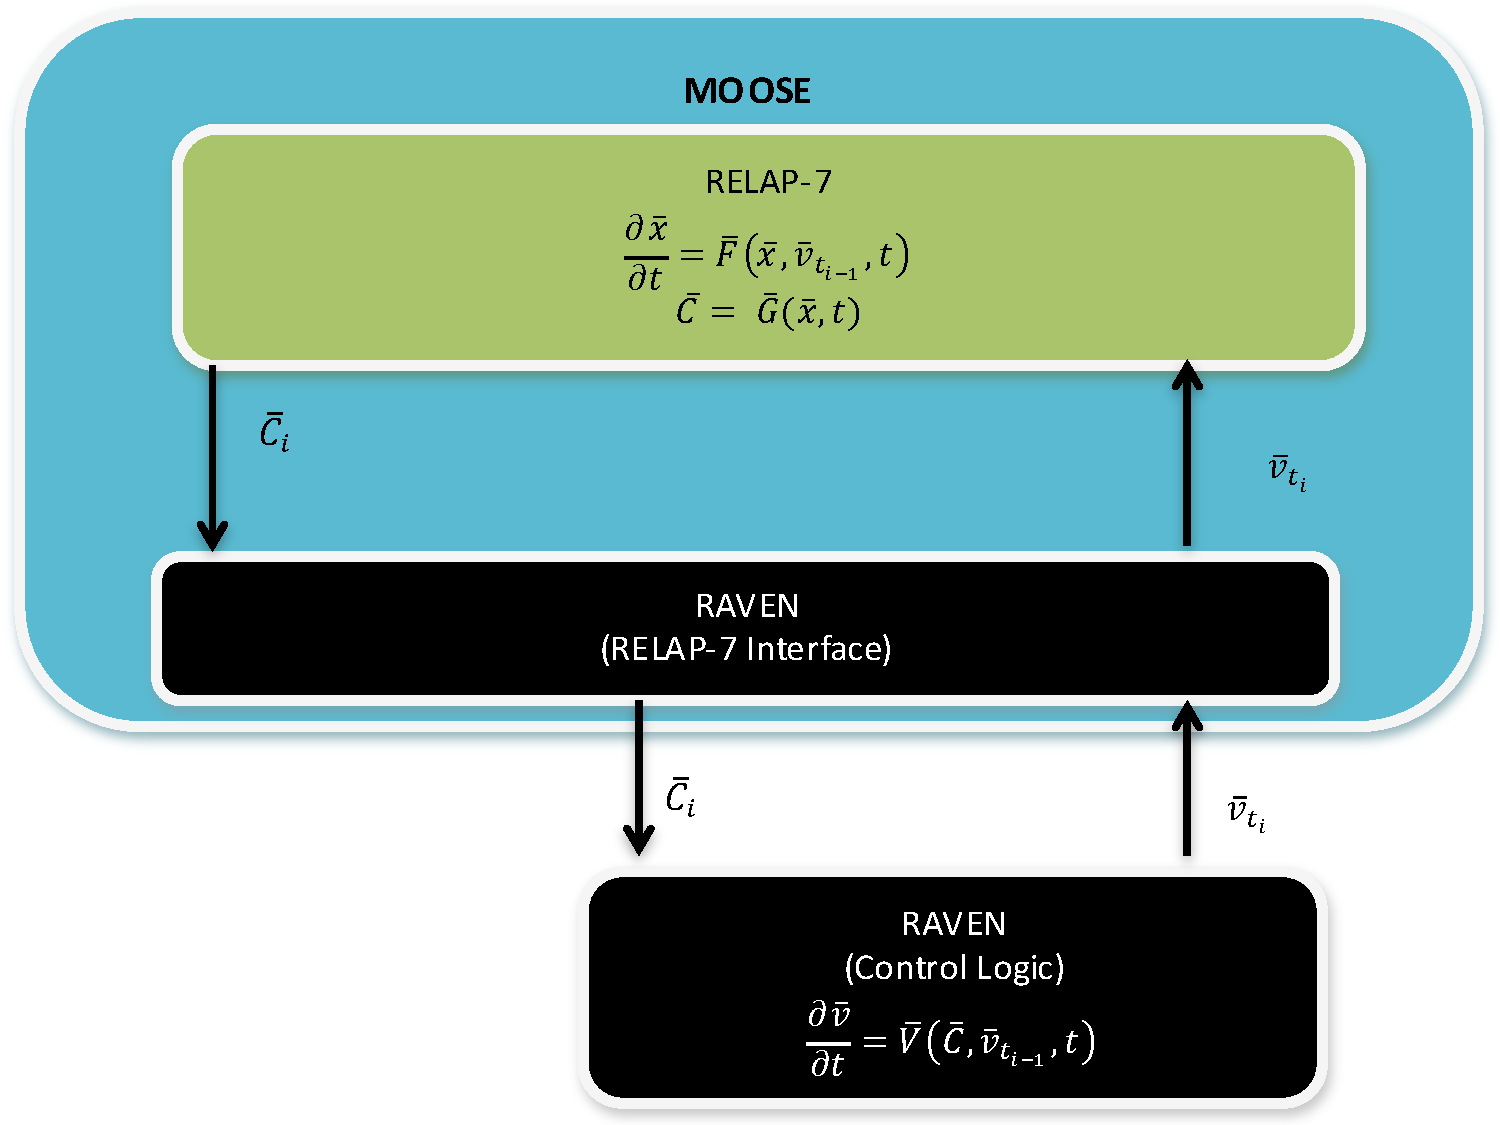
\includegraphics[width=0.5\textwidth]{figures/ControlSystemSoftwareLayout.pdf}
  \caption{Control System Software Layout.}
   \label{fig:ControlSoftwareLayout}
\end{figure}
%%%%%%%%%%%%%%%%%%%%%%%%%%%%%%
\Subsection{The auxiliary plant and component status variables}
%%%%%%%%%%%%%%%%%%%%%%%%%%%%%%
\label{sec:auxiliary}
So far it has been assumed that all information needed is contained in $\bar{x}$ and $\bar{v}$. Even if this information is sufficient for the calculation of the system status in every point in time, it is not a practical and efficient way to implement the control system.
In order to facilitate the implementation of the control logic, a system of auxiliary variables has been introduced .
The auxiliary variables are those that in statistical analysis are artificially added, when possible, to non-Markovian systems into the phase space to obtain back a Markovian behavior, so that only the information contained in the previous time step is needed to determine the future status of the system.
%These variables can be classified into two types:
%\begin{itemize}
%\item Global status auxiliary control variables (e.g., SCRAM status, time at which scram event %begins, time at which hot shut down event begins)
%\item Component status auxiliary variables (e.g., correct operating status, time from abnormal %event)
%\end{itemize}
Thus, the introduction of the auxiliary system into the mathematical framework leads to the following formulation of the Eq.~\ref{eq:generalSystemEquationwithControlSplitting}:
\begin{equation}
\begin{cases}
\dfrac{\partial \bar{x}}{\partial t} = \bar{F}(\bar{x},\bar{v}_{t_{i-1}},t) \\
\bar{C} = \bar{G}(\bar{x},t) & t_{i-1}\leq t\leq t_{i} = t_{i-1} + \Delta t_{i} \\
\dfrac{\partial \bar{a}}{\partial t} = \bar{A}(\bar{x},\bar{C},\bar{a}_{t_{i-1}},\bar{v}_{t_{i-1}},t) \\
\dfrac{\partial \bar{v}}{\partial t} = \bar{V}(\bar{x},\bar{v}_{t_{i-1}},\bar{a},t)
\end{cases}
\label{eq:generalSystemEquationwithControlSplittingAndAux}
\end{equation}


%%%%%%%%%%%%%%%%%%%%%%%%
%Section{SOFTWARE STRUCTURE}
%%%%%%%%%%%%%%%%%%%%%%%%
%\label{sec:softwareStructure}
%RAVEN is a C++/Python software, coded in an high modular and object-oriented way and based on two software sections:
%\begin{itemize}
%\item MOOSE(\textbf{M}ultiphysics \textbf{O}bject-\textbf{O}riented \textbf{S}imulation \textbf{E}nvironment);
%\item RELAP-7.
%\end{itemize}

%%%%%%%%%%%%%%%%%%%%%%%%%%%%%%
\Section{RELAP-7 AND MOOSE}
%%%%%%%%%%%%%%%%%%%%%%%%%%%%%%
\label{sec:MOOSE/RELAP-7}
MOOSE~\cite{MOOSE} is a computer simulation framework,  developed at Idaho National Laboratory (INL), that simplifies the process for predicting the behavior of complex systems and developing non-linear, multi-physics simulation tools. As opposed to traditional data-flow oriented computational frameworks, MOOSE is based on the mathematical principle of Jacobian-Free Newton-Krylov (JFNK) solution methods. Utilizing the mathematical structure present in JFNK, physics are modularized into “Kernels” allowing for rapid production of new simulation tools. In addition, systems are solved fully coupled and fully implicit by employing physics based preconditioning which allows for great flexibility even with large variance in time scales.
Other than providing the algorithms for the solution of the differential equation, MOOSE also provides all the manipulation tools for the C++ classes containing the solution vector. This framework has been used to construct and develop the Thermo-Hydraulic code RELAP-7, giving an enormous flexibility in the coupling procedure with RAVEN.

RELAP-7 is the next generation nuclear reactor system safety analysis. It will become the main reactor systems simulation toolkit for RISMC (\textbf{R}isk \textbf{I}nformed \textbf{S}afety \textbf{M}argin \textbf{C}haracterization)~\cite{mandelliANS_RISMC} project and the next generation tool in the RELAP reactor safety/systems analysis application series (the replacement for RELAP5). The key to the success of RELAP-7 is the simultaneous advancement of physical models, numerical methods, and software design while maintaining a solid user perspective.
Physical models include both PDEs (Partial Differential Equations), ODEs (Ordinary Differential Equations) and experimental based closure models. RELAP-7 will eventually utilize well posed governing equations for multiphase flow, which can be strictly verified. RELAP-7 uses modern numerical methods which allow implicit time integration, higher order schemes in both time and space and strongly coupled multi-physics simulations.
RELAP-7 is the solver for the plant system except for the control system. Referring to the mathematical formulation, RELAP-7 solves
$\frac{\partial \bar{x}}{\partial t} = \bar{F}(\bar{x},\bar{v}_{t_{i-1}},t)$.

%The nuclear power plant is represented and modeled by a set of components (Pipes, Valves, Branches, etc.) and each component type corresponds to a C++ class.

%%%%%%%%%%%%%%%%%%%%%%%%%%%%%%
\Section{RAVEN}
%%%%%%%%%%%%%%%%%%%%%%%%%%%%%%
RAVEN has been developed in a high modular and pluggable way in order to enable easy integration of different programming languages (i.e., \verb!C++!, \verb!Python!) and coupling with other applications including the ones based on MOOSE. The code consists of four modules:
\begin{itemize}
\item RAVEN/RELAP-7 interface (see Section~\ref{sec:interface})
\item \verb!Python! Control Logic (see Section~\ref{sec:pythonControlLogic})
\item \verb!Python! Calculation Driver (see Section~\ref{sec:pyhtonCalcDriver})
\item Graphical User Interface (see Section~\ref{sec:GUI})
\end{itemize}

%%%%%%%%%%%%%%%%%%%%%%%%%%%%%%
\Subsection{RAVEN/RELAP-7 interface}
\label{sec:interface}
%%%%%%%%%%%%%%%%%%%%%%%%%%%%%%
The RAVEN/RELAP-7 interface, coded in \verb!C++!, is the container of all the tools needed to interact with RELAP-7/MOOSE. It has been designed in order to be general and pluggable with different solvers simultaneously in order to allow an easier and faster development of the control logic/PRA capabilities for multi-physics applications.
The interface provides all the capabilities to control, monitor, and process the parameters/quantities in order to drive the RELAP-7/MOOSE calculation. In addition, it contains the tools to communicate to the MOOSE input parser which information, i.e. input syntax, must be provided in order to run a RAVEN  calculation. So far, the input file includes four main sections.:
\begin{itemize}
\item \emph{RavenMonitored} class;
\item \emph{RavenControlled} class;
\item \emph{RavenAuxiliary} class;
\item \emph{RavenDistributions} class.
\end{itemize}
%%%
% Monitored and Controlled
%%%
The \emph{RavenMonitored} and \emph{RavenControlled}  classes provide the connection with the calculation framework in order to retrieve the post-processed quantities (e.g., Monitored = average fuel temperature, etc.) and to fetch and/or perturb parameters (e.g., Controlled = pump mass flow, etc.) within the simulation. The typical input structure for Monitored and Controlled parameters in RAVEN is as following:
\begin{lstlisting}
[Controlled]
  control_logic_input = control_logic_input_file_name
  [./power_fraction_CH1]
    property_name = FUEL:power_fraction
    data_type = double
    component_name = CH1
  [../]
  ...
[]
\end{lstlisting}
\begin{lstlisting}
[Monitored]
  [./MaxTempCladCH1]
    component_name = CH1
    operator = NodalMaxValue
    property_name = CLAD:TEMPERATURE
    data_type = double
  [../]
  ...
[]
\end{lstlisting}

Within the blocks identified by the keywords \textbf{Monitored} and \textbf{Controlled}, the user can specify the monitored quantities that need to be processed during the calculation and the parameters that will be controlled through the \verb!Python! control logic. The name and path of the control logic input file are provided by the keyword  \textbf{control\_logic\_input} (not specifying the ".py" extension). Each monitored and controlled variable is identified through a \textbf{Raven Alias} (i.e., MaxTempCladCH1, power\_fraction\_CH1), the name that is used in the control logic \verb!Python! input in order to refer to the variable contained in the simulation.
The user has to provide the following information in order to build a Raven variable:
\begin{itemize}
  \item \textbf{component\_name}, the name of the RELAP-7 component that contains the variable the code must act on;
  \item \textbf{operator} (only for Monitored variables), the post-processor operation that must be performed on the variable;
  \item \textbf{property\_name}, the variable name and its location within the calculation framework (RELAP-7/MOOSE variable name);
  \item \textbf{data\_type}, data type (i.e., double, float, int, boolean).
\end{itemize}
RAVEN can use all the post-processor operators that are available in MOOSE (e.g., ElementAverageValue, NodalMaxValue, etc.). Depending on which component it's acting on, some operations may be disabled (for example,  ElementAverageValue is not available in 0-D components).
%%%%
%% Controlled
%%%%
%
%The \emph{RavenControlled} class provides the link between RAVEN and RELAP-7/MOOSE in order to retrieve and/or change properties within the simulation (e.g., fuel thermal conductivity, pump mass flow). The typical input structure for a controlled parameter in RAVEN is as follows:
%\begin{lstlisting}
%[Controlled]
%  control_logic_input = control_logic_input_file_name
%  [./power_fraction_CH1]
%    property_name = FUEL:power_fraction
%    data_type = double
%    component_name = CH1
%  [../]
%  [./power_fraction_CH2]
%    property_name = FUEL:power_fraction
%    data_type = double
%    component_name = CH2
%  [../]
%  ...
%[]
%\end{lstlisting}
%Within the block identified by the keyword \textbf{Controlled}, the user can specify the properties that, during the calculation, will be controlled through the \verb!Python! control logic. The name and path of the control logic input file are provided by the parameter  \textbf{control\_logic\_input} (not specifying the ".py" extension). Each controlled variable is identified through a \textbf{Raven Alias} (e.g., power\_fraction\_CH1): the name that is used in the control logic \verb!Python! input in order to refer to the parameter contained in the simulation.
%The user has to provide different information in order to build a controlled variable:
%\begin{itemize}
%  \item \textbf{component\_name}, the name of the RELAP-7 component that contains the variable the code must act on;
%  \item \textbf{property\_name}, the variable name and its location within the calculation framework (RELAP-7/MOOSE variable name);
%  \item \textbf{data\_type}, data type (i.e., double, float, int, boolean).
%\end{itemize}
%Through this class, RAVEN is able to retrieve property values and, in case of changes, push the new values back into the simulation.
%%%
% Auxiliary
%%%

The \emph{RavenAuxiliary} class is the container of auxiliary variables. The Raven Auxiliary system is not connected with RELAP-7/MOOSE environment. The typical input structure for a auxiliary parameter in RAVEN is as follows:
\begin{lstlisting}
[RavenAuxiliary]
  [./scram_start_time]
    data_type     = double
    initial_value = 61.0
  [../]
  ...
[]
\end{lstlisting}
%Each auxiliary variable is identified through a \textbf{Raven Alias} (e.g., CladDamaged): the name that is used in the control logic \verb!Python! input in order to refer to the parameter contained in the RAVEN interface.
In addiction to the data type, in order to construct an auxiliary variable, the user needs to provide an initial value.
%\begin{itemize}
%  \item \textbf{initial\_value}, initialization value;
%  \item \textbf{data\_type}, data type (i.e., double, float, int, bool).
%\end{itemize}
As previously mentioned, these variables are needed to ensure that the system remains Markovian, so that only the previous time step information are necessary to determine the future status of the plant.
%%%
% Distributions
%%%

The \emph{RavenDistributions} class contains the algorithms, structures and interfaces for several predefined probability distributions. It is only available in the \verb!Python! control logic, since it is not needed a direct interaction with RAVEN/RELAP-7/MOOSE environment. The user can actually choose among nine different types of distribution (e.g., Normal, Triangular, Uniform, Exponential); each of them, in order to be initialized, requires a different set of parameters depending on the type of distribution.
As an example, the following input create a Normal and a Triangular distribution:
\begin{lstlisting}
[Distributions]
  [./ExampleNormalDis]
    type =  NormalDistribution
    mu = 1
    sigma = 0.01
    xMax = 0.8
    xMin = 0
  [../]
  [./ExampleTriangularDis]
    type   = TriangularDistribution
    xMin  = 1255.3722
    xPeak = 1477.59
    xMax  = 1699.8167
  [../]
  ...
[]
\end{lstlisting}
The class RavenDistributions is the base of the Monte-Carlo and Dynamic Event Tree capabilities present in RAVEN.
%%%%%%%%%%%%%%%%%%%%%%%%%%%%%%
\Subsection{Python Control Logic}
\label{sec:pythonControlLogic}
%%%%%%%%%%%%%%%%%%%%%%%%%%%%%%
The control logic module is used to drive a RAVEN/RELAP-7 calculation. Up to now it is implemented by the user via \verb!Python! scripting. The reason of this choice is to try to preserve generality of the approach in the initial phases of the project so that further specialization is possible and  inexpensive.
The form through which the RAVEN variables can be called is the following:
\begin{itemize}
  \item Auxiliary.RavenAlias;
  \item Controlled.RavenAlias;
  \item Monitored.RavenAlias.
\end{itemize}
Regarding the RavenDistributions mentioned in Section 4.1, they are also available for the control logic in a similar form to the other variable (distributions.RavenAlias(allowable list of arguments) ).
The implementation of the control logic via \verb!Python! is rater convenient and flexible. The user only needs to know few \verb!Python! syntax rules in order to build an input. Although this extreme simplicity, it will be part of the GUI task to automatize the construction of the control logic scripting in order to minimize user effort.
\\A small example of a control logic input is reported below: the thermal conductivity of the gap (thermalConductGap) is set equal to the thermal conductivity of the fuel when the fuel temperature (averageFuelTemperature) is greater than 910 K.
\lstset{
   language=Python,
   showstringspaces=false,
   formfeed=\newpage,
   tabsize=2,
   commentstyle=\itshape
}
\begin{lstlisting}
import sys
def control_function(monitored, controlled):
    if monitored.averageFuelTemperature > 910:
        controlled.thermalConductGap = controlled.thermalConductFuel
    return
\end{lstlisting}

%%%%%%%%%%%%%%%%%%%%%%%%%%%%%%
\Subsection{Python Calculation Driver}
\label{sec:pyhtonCalcDriver}
%%%%%%%%%%%%%%%%%%%%%%%%%%%%%%
Analysis of dynamic stochastic systems can be extremely challenging due to the complexity and high dimensionality of the system solving equations. An analytical solution is only available for rather simple cases. When an analytical solution is not available, numerical methods are often employed.
%In order to solve the system governing equations, two main approaches can be followed:
%\begin{itemize}
%\item Determine approximate solutions of the exact problems;
%\item Determine the exact solution for the approximate models.
%\end{itemize}
%Due to the very large complexity and the high dimensionality of the systems considered,
Hence, RAVEN employs a Monte-Carlo based algorithm.
The main idea is to run a set of simulations having different dynamic and static uncertainty of physical parameters, presence of noise and initial conditions and terminate them when one of the following stopping conditions are reached:
\begin{itemize}
\item Mission time (i.e., an user specified end time);
\item Main event (i.e., maximum temperature of the clad or core damage).
\end{itemize}
These algorithms have been implemented in the \verb!Python! module called "Raven Runner''. It consists in a \verb!Python! driver which calls RAVEN multiple times, changes initial conditions and seeds the random generator for the distributions.
The multiple calculations, required by the employment of these algorithms, can be run in parallel, using queues/sub-process/\verb!Python! systems.

\begin{figure}[h]
\centering
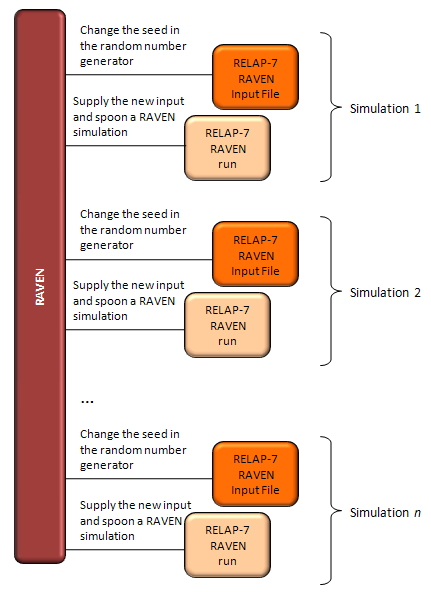
\includegraphics[width=0.4\textwidth]{figures/sampling_mc.PNG}
\caption{Monte-Carlo sampling scheme.}
\label{fig:MCsampling}
\end{figure}

The analysis of dynamic stochastic systems through Monte-Carlo algorithm can be summarized (Figure~\ref{fig:MCsampling}) as follows:
\begin{enumerate}
\item Initial Sampling of:
       \begin{enumerate}
       \item Physical parameters
       \item Initial conditions
       \item Transition conditions, i.e. time instant in which transition events occur (e.g., time in which a reactor scram occurs, time delta to recover power grid)
    \end{enumerate}
\item Run the system simulator using the values previously sampled and eventually applying a random noise to some parameters at each time step
\item Repeat steps 1-2 for a large number of calculations (user input)
\end{enumerate}
Figure~\ref{fig:MCsampling} shows a scheme of the interaction between the code and the RAVEN runner in case of Monte-Carlo calculations. The runner basically perform a different seeding of the random number generator and interact, through RAVEN, with the \verb!Python! control logic input in order to sample the variables specified by the user.
%%%%%%%%%%%%%%%%%%%%%%%%%%%%%%
\Subsection{Graphical User Interface}
\label{sec:GUI}
%%%%%%%%%%%%%%%%%%%%%%%%%%%%%%
As previously mentioned, a Graphical User Interface (GUI) is not required to run RAVEN, but it represents an added value to the whole code. The GUI is compatible with all the capabilities actually present in RAVEN (control logic, Monte-Carlo, etc.).  Its development is performed using QtPy, which is a \verb!Python! interface for a \verb!C++! based library for GUI implementation. The GUI is based on a software named Peacock, which is a GUI interface for MOOSE based application and, in its base implementation, is only able to assist the user in the creation of the input.  In order to make it fit all the RAVEN needs, the GUI has been specialized and it is in continuous evolution. Figure ~\ref{fig:RavenGUI} shows the input tab of the RAVEN GUI. Through the box on the left the user is able to construct the RAVEN/RELAP-7 input or modify parameters/components already inputted. On the right side, the 3D layout of the plant is drawn.
\begin{figure}[h]
   \centering
    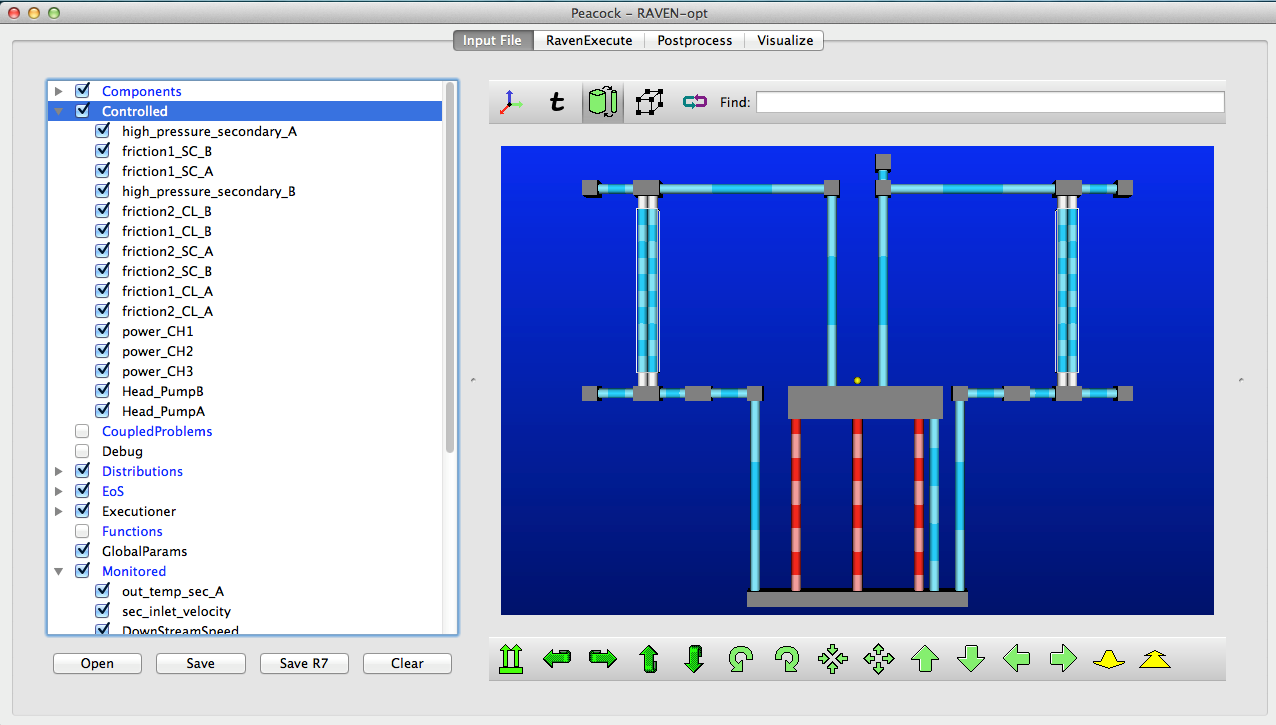
\includegraphics[width=0.8\textwidth]{figures/RavenGUI.PNG}
    \caption{Input/plan Visualization GUI Window.}
    \label{fig:RavenGUI}
\end{figure}
%%%%%%%%%%%%%%%%%%%%%%%%%%%%%%
\Section{SOFTWARE LAYOUT AND CALCULATION FLOW}
\label{sec:swLayoutCalcFlow}
%%%%%%%%%%%%%%%%%%%%%%%%%%%%%%
\begin{figure}
  \centering
     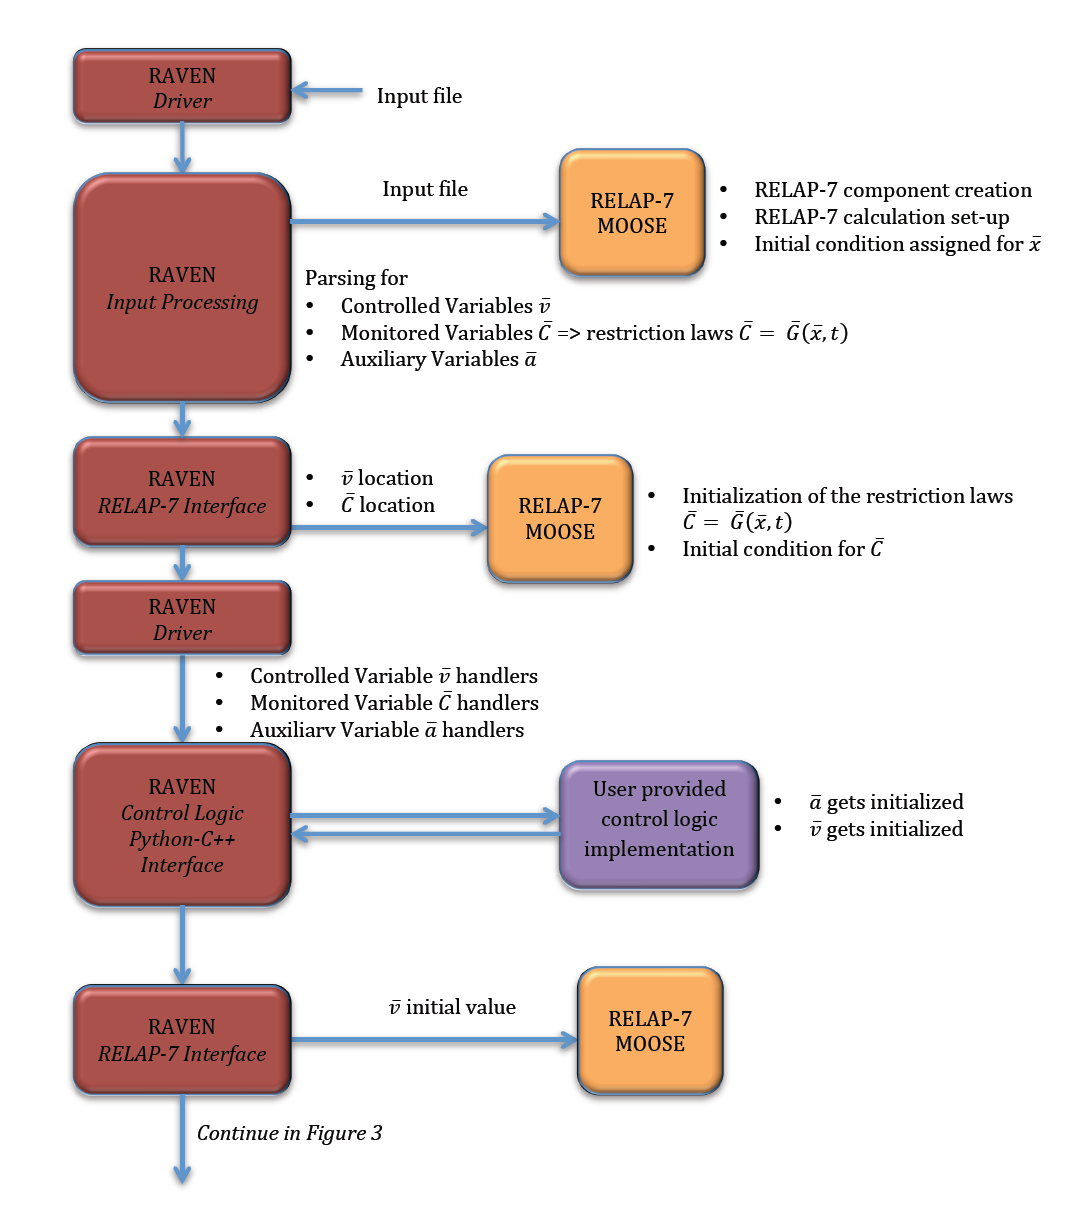
\includegraphics[width=1\textwidth]{figures/CalculationFlow_part_1.PNG}
  \caption{RAVEN Calculation Flow - Initialization.}
  \label{fig:CalcFlow1}
\end{figure}

\begin{figure}
  \centering
     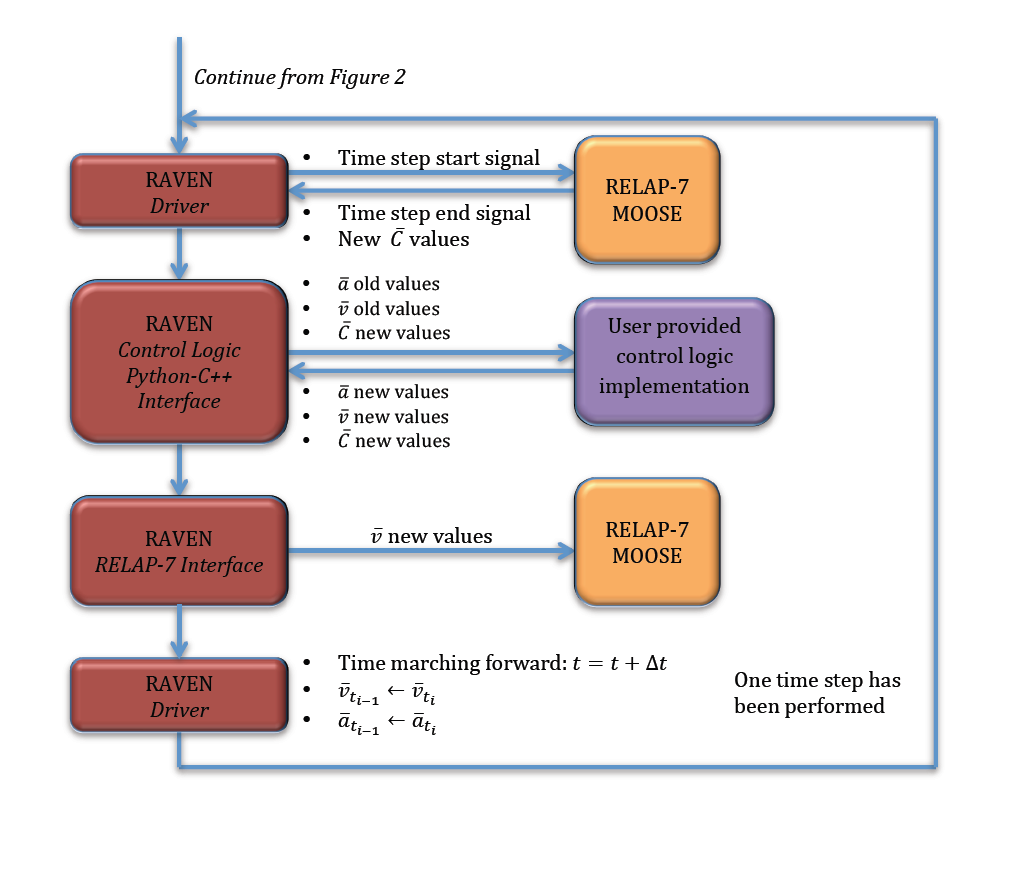
\includegraphics[width=1\textwidth]{figures/CalculationFlow_part_2.PNG}
  \caption{RAVEN Calculation Flow - Run.}
  \label{fig:CalcFlow2}
\end{figure}
Figures~\ref{fig:CalcFlow1} and \ref{fig:CalcFlow2} show the calculation flow employed by RAVEN/RELAP-7/MOOSE software.
A typical RAVEN calculation can be summarized in the following logic steps:
\begin{enumerate}
   \item Perform Initialization
   \item RELAP-7/MOOSE updates the information contained in each component class with the actual solution $\bar{x}$
   \item RAVEN requests MOOSE to perform the post-processing manipulation in order to construct $\bar{C}$
   \item Equation
$\frac{\partial \bar{v}}{\partial t} = \bar{V}(\bar{x},\bar{v}_{t_{i-1}},t) $
is solved and the set of control parameters for the next time step $v_{t_{i}}$ is determined
  \item RAVEN asks RELAP-7/MOOSE to compute the solution $\bar{x}$ for the following time step
  \item Repeat from 2 to 5 until the end of the calculation or an exit condition is reached (e.g., clad failure)
\end{enumerate}

%%%%%%%%%%%%%%%%%%%%%%%%
\Section{DEMO FOR A PWR PRA ANALYSIS}
%%%%%%%%%%%%%%%%%%%%%%%%
In order to show the capabilities of RAVEN coupled with RELAP-7/MOOSE, a simplified PWR PRA analysis has been employed.
\begin{figure}[h]
   \centering
    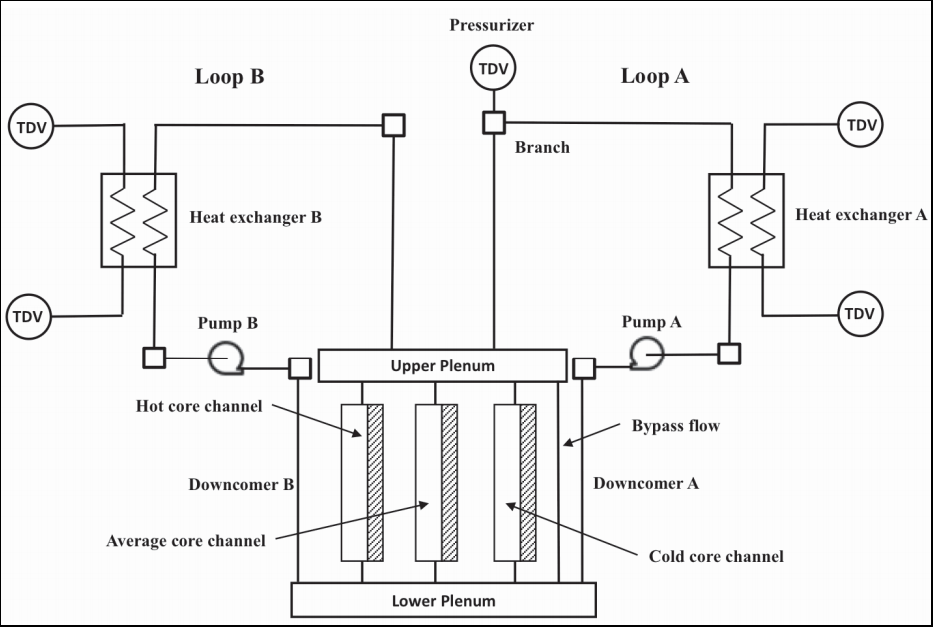
\includegraphics[width=0.5\textwidth]{figures/PWR_TMI_SCHEME.PNG}
    \caption{PWR model scheme.}
    \label{fig:PWRmodel}
\end{figure}
Figure~\ref{fig:PWRmodel} shows the scheme of the PWR model. The reactor vessel model consists of the Down-comers, the Lower Plenum, the Reactor Core Model and the Upper Plenum. Core channels (flow channels with heat structure attached to each of them) were used to describe the reactor core. The core model consists of three parallel core channels and one bypass flow channel.
%The hot core channel represents the inner hottest zone of the reactor core. The average core channel represents the mid zone of the core and the cold core channel represents the outer zone of the core, respectively.
There are two primary loops, i.e., loop A and loop B. Each loop consists of the Hot Leg, a Heat Exchanger and its secondary side pipes, the Cold Leg and a primary Pump. A Pressurizer is attached to the Loop A piping system to control the system pressure. A Time Dependent Volume (pressure boundary conditions) component is used to represent the Pressurizer. Since the RELAP-7 code does not have the two-phase flow capability yet, single-phase counter-current heat exchanger models are implemented to mimic the function of steam generators in order to transfer heat from the primary to the secondary.
In order to perform a PRA analysis on this simplified model, it has been necessary to control unconventional parameters (i.e. inlet/outlet friction factors), since RELAP-7 still has limitations for the component controllable parameters and models. In the following paragraph, the PRA station black out sequence of events is reported.
%%%%%%%%%%%%%%%%%%%%%%%%%%%%%%
\Subsection{Station Black Out (SBO) analysis}
%%%%%%%%%%%%%%%%%%%%%%%%%%%%%%
The Probabilist Risk Assessment analysis has been performed simulating a Station Black Out accident, making Monte-Carlo samplings on the recovery time of the diesel generators  $t_{1}$ (delta time from reactor scram signal) and the clad failure temperature $TC{f}$. Two sets of Monte-Carlo calculations have been run:
 \begin{itemize}
   \item 400 runs, randomizing $t_{1}$ (Normal distribution, mu = 120 s, sigma = 20 s) and $TC{f}$ (Triangular distribution, xPeak = 1477.59\footnote{Typical PRA success criteria.} K, xMin~ =~1255.37\footnote{10 CFR50.46 limit.} K, xMax = 1699.82 K~\cite{Urbanic1978})
   \item 400 runs, randomizing only $t_{1}$
\end{itemize}
The SBO transient is based on the following sequence of events (starting from a steady-state operational condition of the Nuclear Power Plant~\cite{relap7FY12}):
 \begin{itemize}
   \item 60.0 seconds, transient begins
   \item 61.0 seconds, loss of power grid and immediate shutdown of the reactor(scram):
   \begin{itemize}
       \item Pump coast-down;
       \item Decay heat power;
       \item Diesel Generators and residual heat removal system (RHRS) not available.
    \end{itemize}
   \item $t_{1}$, recovery of the diesel generators
   \item $t_{2}$, end of transient either for clad failure or 300 seconds of simulation (PRA success)
\end{itemize}
Since the scope of this demo is to show the capabilities contained in RAVEN and RELAP-7 capabilities are not optimized for long simulation times, the transient has been accelerated in order to simulate a maximum of 300 seconds.
In the following paragraph, the simulations results are shown and explained.
%%%%%%%%%%%%%%%%%%%%%%%%%%%%%%
\Subsection{Results}
%%%%%%%%%%%%%%%%%%%%%%%%%%%%%%

Figure~\ref{fig:distributionResults} shows the distribution of the maximum temperature reached by the clad in the core channels (blue histogram) and compares it with the distribution of clad failure temperature (red histogram).
%Although there is large overlapping of the two distributions, which indicates a high failure probability of the system considered, the scope of the analysis was just to show  RAVEN capabilities to perform stochastic analysis of relatively complex systems.
The distribution of the clad temperature already accounts for the simulations that have been stopped for having reached the corresponding failure temperature. Therefore, the overlapping of the two distributions is not representative of the total failure rate. Instead, the total failure rate could be inferred from the steep decrease on the higher temperature side of the number of counts with respect the lower temperature one. The probability of failure is artificially elevated with respect a real case in order to keep the effort bounded while illustrating the full RAVEN capabilities.

\begin{figure} [H]
\centering
\begin{subfigure}{.5\textwidth}
  \centering
  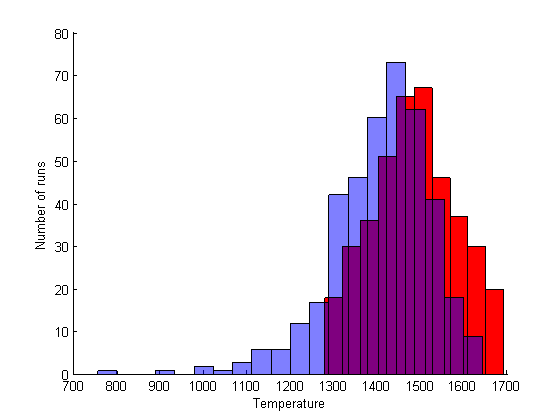
\includegraphics[width=1\linewidth]{figures/PRA_dist1.png}
  \label{fig:runs_temp_dist}
\end{subfigure}%
\begin{subfigure}{.5\textwidth}
  \centering
  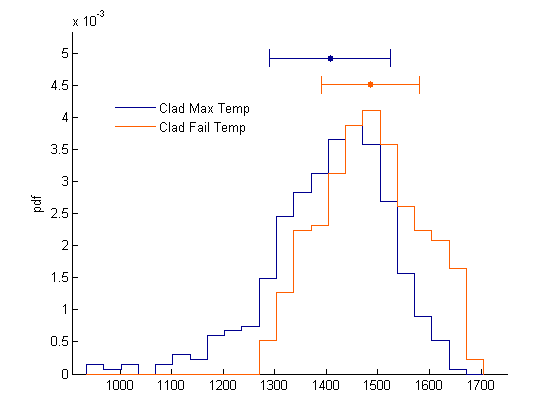
\includegraphics[width=1\linewidth]{figures/PRA_dist2.png}
  \label{fig:pdf_temp}
\end{subfigure}
\caption{Comparison between max reached clad temperature and clad failure temperature distributions: binning results (left) and associated probability distribution functions (right)}
\label{fig:distributionResults}
\end{figure}
In addition, Fig.~\ref{fig:limit_surface_rng_temp_and_dg} shows the limit surface, i.e. the boundaries between system failure (red points) and system success (green points), obtained by the $400$ Monte-Carlo simulations. Since only two uncertain parameters have been considered (i.e., DG recovery time and clad fail temperature), this boundary lies in a 2-dimensional space.
The slope of the limit surface pictured in Fig.~\ref{fig:limit_surface_rng_temp_and_dg} also shows, in this particular demo, how the DG recovery time has a greater impact on the system dynamics then the clad failure temperature (this is confirmed also when rescaling the Fig.~\ref{fig:limit_surface_rng_temp_and_dg} in term of relative deviation from the average values).

\begin{figure}[h]
   \centering
    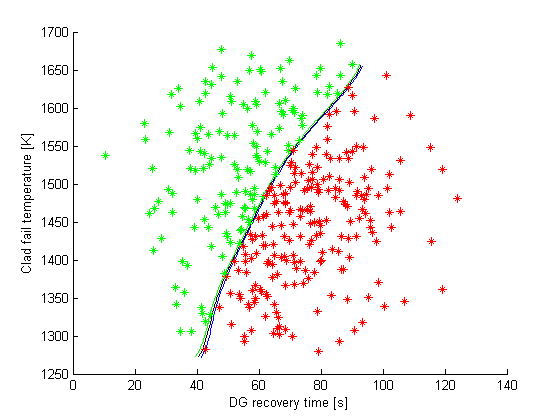
\includegraphics[width=0.6\textwidth]{figures/PRA_limitSurface.png}
    \caption{Limit Surface for the SBO analysis of a simplified PWR model}
    \label{fig:limit_surface_rng_temp_and_dg}
\end{figure}

It has also been performed a new set of $400$ Monte-Carlo simulations in which, now, the clad failure temperature is fixed at a predefined value $T_{Fail}=1477.59$ (i.e., there is no triangular distribution associated to it). As expected, the numberof simulations that let to system failure was slightly different among these two sets of simulations: $203$ for the first case and $224$ for this last one.This fact shows how modeling of uncertainties can impact risk evaluation.

%%%%%%%%%%%%%%%%%
\section{CONCLUSIONS}
%%%%%%%%%%%%%%%%%
In this paper it has been presented RAVEN as a tool to perform dynamic PRA through Monte-Carlo sampling. In particular, the software structure and all the components that are involved in the computation have been presented, including system simulator (i.e., RELAP-7) and the control logic, characterized by monitor system dynamics and on-line control of selected parameters.
An example of PRA analysis has been also presented for a SBO-like case for a simplified PWR loop.
The description of the implementation for such case demonstrates how the flexibility of the software framework provides the basic tools to perform Dynamic PRA, uncertainty quantification and plant control.
Next capabilities, to be implemented to RAVEN and that are currently under development, include dynamic event tree generation~\cite{ADAPTHakobyan}, adaptive sampling~\cite{mandelliSVMANS} and more advanced data mining algorithms~\cite{mandelliEsrel2011}.
%%%%%%%%%%%%%%%%%%%%%%%%%%%%%%%%%%%%%%%%%%%%%%%%%%%%%%%%%%%%%%%%%%%%%%%%%%%%%%%%
\section*{ACKNOWLEDGMENT}
%%%%%%%%%%%%%%%%%%%%%%%%%%%%%%%%%%%%%%%%%%%%%%%%%%%%%%%%%%%%%%%%%%%%%%%%%%%%%%%%
This work is supported by the U.S. Department of Energy, under DOE Idaho Operations Office Contract DE-AC07-05ID14517. Accordingly, the U.S. Government retains a nonexclusive, royalty-free license to publish or reproduce the published form of this contribution, or allow others to do so, for U.S. Government purposes.

\bibliographystyle{ieeetr}
\bibliography{bibl}


\end{document}


